\documentclass{article}
\usepackage{graphicx} % Required for inserting images
\usepackage{graphicx} % Required for inserting images
\usepackage[left=1.5cm, right=1.5cm, top=1cm, bottom=1.5cm]{geometry}
\usepackage{amsmath}
\usepackage{amssymb}
\usepackage{amsfonts}
\usepackage{amsthm}
\usepackage{ulem}
\usepackage{bm}
\usepackage{tikz}
\usepackage{enumitem}
\usetikzlibrary{shapes,backgrounds}
\usepackage{textcomp} % for \textdollar command

\date{}

\begin{document}
\fontsize{12}{13} \selectfont %This is 12pt text with 14pt line spacing.
%\setcounter{page}{2}

\begin{center}
Potterhouse School \hspace{3cm} Year 6 Math - Homework - Term 1 - Week 13 - Task (iii) 
\end{center}

\begin{enumerate}
    \item  \quad Find the perimeter and are of the shape below. 
\begin{center} 
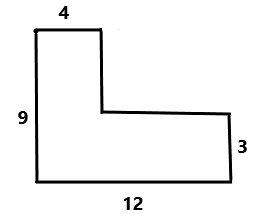
\includegraphics[width=5cm]{Year_6_Mixed_Tests/Homework_Tasks/cpd_shp_2.png}
\end{center}

\\
(a) Perimeter \\
(b) Area \\

\item \quad Find the volume of the shape below. \\
\begin{center}
    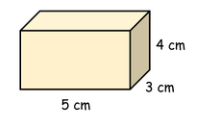
\includegraphics{Year_6_Mixed_Tests/Homework_Tasks/Cuboid_vol.png}
\end{center}
\\

\item \quad (a) Give the number of fruits from the bar chart. \\
\begin{center}
    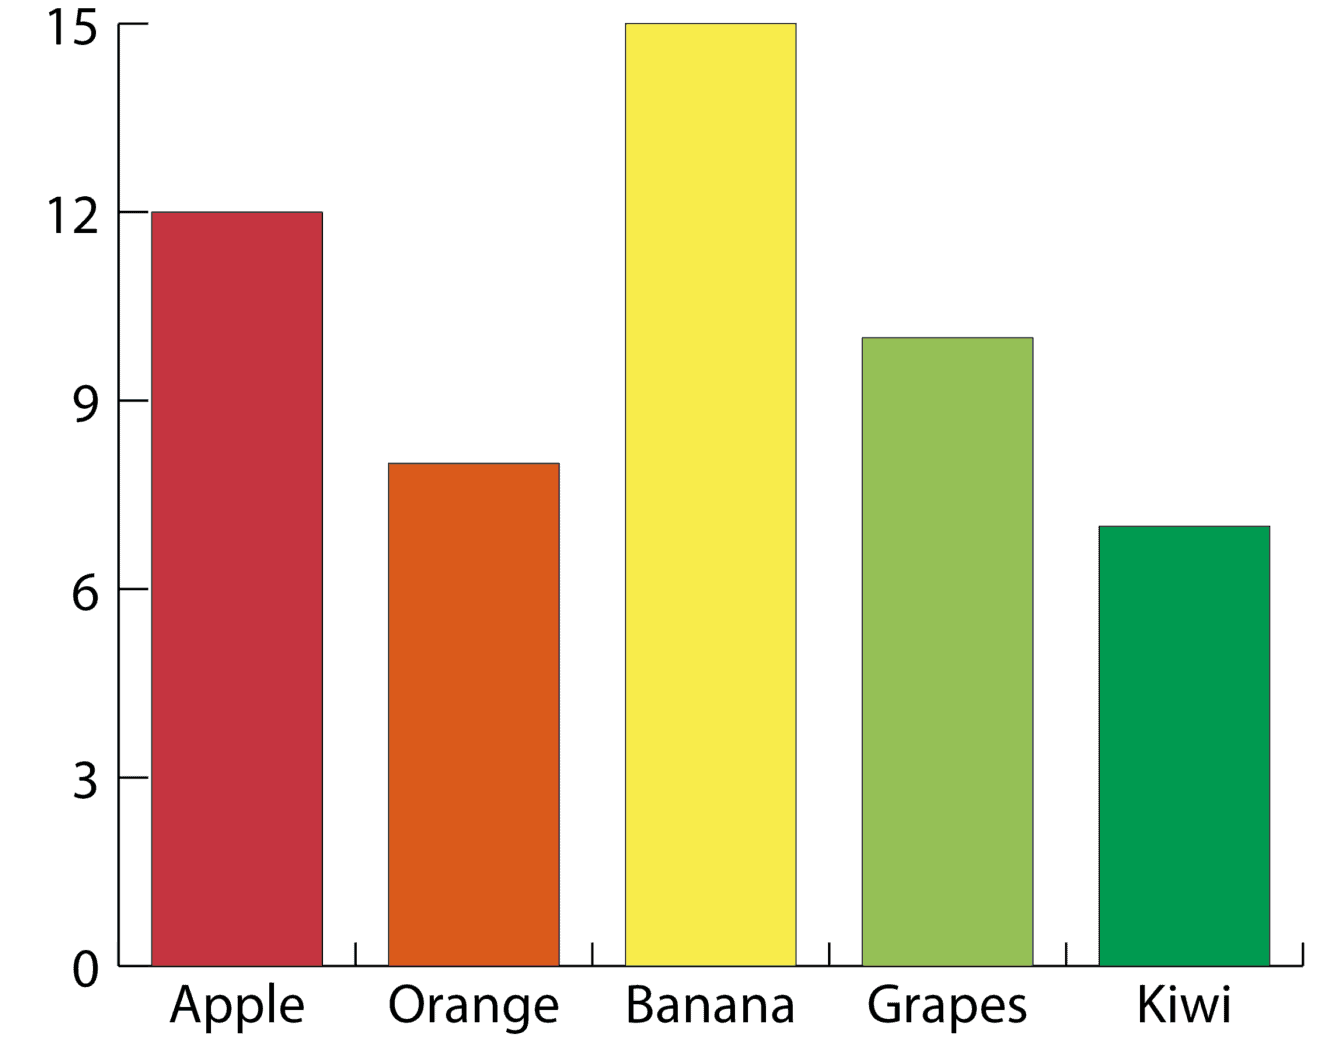
\includegraphics[width=7cm]{Year_6_Mixed_Tests/Homework_Tasks/Bar_chart_2.png}
\end{center}
\\

(i) Apples \\
(ii) Oranges \\
(iii) Bananas \\
(iv) Grapes \\
(v) Kiwi \\ 

(b) Label the y-axis appropriately. \\
(c) Give the chart a title.


    
\end{enumerate}




\end{document}
